\documentclass[letter,12pt]{article}
\usepackage{ifpdf}
\makeatletter
\edef\texforht{TT\noexpand\fi
  \@ifpackageloaded{tex4ht}
    {\noexpand\iftrue}
    {\noexpand\iffalse}}
\makeatother
\ifpdf
  \usepackage[framemethod=TikZ]{mdframed}
\else
  \usepackage{framed}
  \def\pgfsysdriver{pgfsys-tex4ht-alt.def}
\fi
\title{PHYS 704 \\ Homework 5}
\author{Daniel Pad\'e}
\date{March 2, 2016}

\usepackage{enumerate}
\usepackage{amsfonts}
\usepackage{amsmath}
\usepackage{amssymb}
\usepackage{amsthm}
\usepackage{mathtools}
\usepackage{bm}
\usepackage{graphicx}
\usepackage{fancyhdr}
\usepackage{tikz}
\usepackage{float}
\usetikzlibrary{arrows}


\pagestyle{fancy}
\fancyhf{}
\fancyhead[LE,RO]{Daniel Pad\'e}
\fancyhead[RE,LO]{PHYS 704}
\fancyhead[CE,CO]{Homework 5}

\fancyfoot[LE,RO]{\thepage}

\theoremstyle{definition}
\newtheorem*{sol}{Solution}

\begin{document}
\maketitle
\begin{enumerate}
    \item
        \begin{enumerate}
            \item
                Construct the free-space Green function $G(x, y; x',
                y')$ for two-dimensional electrostatics by integrating
                $1/R$ with respect to $(z' - z)$ between the limits
                $\pm Z$ where $Z$ is taken to be very large. Show that
                apart from an inessential constant, the Green function
                can be written alternately as
                \begin{align*}
                    G(x, y; x', y') &= - \ln \left[ {(x - x')}^2 + {(y - y')}^2 \right]
                    \\
                    &= - \ln \left[ \varrho^2 + \varrho'^2 - 2 \varrho \varrho' \cos( \phi - \phi' )\right]
                \end{align*}
                \begin{sol}
                    Use the following definitions:
                    \begin{align*}
                        \alpha &\coloneqq \sqrt{{(x - x')}^2 + {(y - y')}^2}
                        \\
                        u &\coloneqq z - z'
                    \end{align*}
                    to integrate
                    \begin{align*}
                        \int_{-Z}^{Z} \frac{du}{\sqrt{\alpha^2 + u^2}}
                        &= \ln \left( \sqrt{\alpha^2 + u^2} + u \right) \biggr \rvert_{-Z}^{Z}
                        \\
                        &= \ln \frac{\sqrt{Z^2 + \alpha^2} + Z}{\sqrt{Z^2 + \alpha^2} - Z}
                        \\
                        &= \ln \frac{\sqrt{1 + \frac{\alpha^2}{Z^2}} + 1}{\sqrt{1 + \frac{\alpha^2}{Z^2}} - 1}
                    \end{align*}
                    Expanding to first order in $\frac{\alpha^2}{Z^2}$ yields
                    \begin{align*}
                        G &= \ln \frac{2 + \frac{\alpha^2}{2 Z^2}}{\frac{\alpha^2}{2Z^2}}
                        \\
                        &= \ln \frac{4Z^2 + \alpha^2}{\alpha^2}
                        \\
                        &= \ln \left(4Z^2 + \alpha^2\right) - \ln \alpha^2
                        \\
                        G(Z \gg \alpha) &= \ln 4Z^2 - \ln \alpha^2
                    \end{align*}
                    \begin{align*}
                        \therefore
                        G(x, y; x', y') &= - \ln \alpha^2
                        \\
                        &= - \ln \left[{(x - x')}^2 + {(y - y')}^2\right]
                    \end{align*}
                    Changing to cylindrical coordinates yields
                    \begin{align*}
                        G(x, y;x',y') &= - \ln \left[ \varrho^2 + \varrho'^2 - 2 \varrho \varrho' \cos( \phi - \phi' )\right]
                    \end{align*}
                \end{sol}
            \item
                Show explicitly by separation of variables in polar
                coordinates that the Green function can be expressed
                as a Fourier series in the azimuthal coordinate,
                \begin{align*}
                    G = \frac{1}{2 \pi} \sum_{-\infty}^{\infty} e^{i m (\phi - \phi')}g_m(\varrho, \varrho')
                \end{align*}
                where the radial Green functions satisfy
                \begin{align*}
                    \frac{1}{\varrho'}\frac{\partial}{\partial \varrho'}
                    \left(
                        \varrho' \frac{\partial g_m}{\partial \varrho'}
                    \right)
                    - \frac{m^2}{\varrho'^2} g_m
                    =
                    - 4 \pi \frac{\delta(\varrho - \varrho')}{\varrho}
                \end{align*}
                Note that $g_m(\varrho, \varrho')$ for fixed $\varrho$
                is a different linear combination of the solutions of
                the homogenous radial equation (2.68) for $\varrho' <
                \varrho$ and for $\varrho' > \varrho$, with a
                discontinuity of slope at $\varrho' = \varrho$
                determined by the source delta function
                \begin{sol}
                    The defining equations of the greens function
                    \begin{align*}
                        \int_\Omega \nabla'^2 G(\varrho, \phi;\varrho', \phi') \varrho' d\varrho' d\phi' = -4 \pi
                        \\
                        \nabla'^2 G(\varrho, \phi; \varrho', \phi') \propto \delta(\varrho - \varrho')\delta(\phi - \phi')
                    \end{align*}
                    can be satisfied if
                    \begin{align*}
                        \nabla'^2 G = -4\pi \frac{\delta(\varrho - \varrho')\delta(\phi - \phi')}{\varrho}
                    \end{align*}
                    Applying the laplacian to the given expansion yields:
                    \begin{align*}
                        \nabla'^2 G &= \left[
                        \frac{1}{\varrho'}
                        \frac{\partial}{\partial \varrho'}
                        \left(\varrho' \frac{\partial}{\partial \varrho'}\right)
                        - \frac{1}{\varrho'^2}\frac{\partial}{\partial \phi'^2}
                    \right]
                    \left[
                        \frac{1}{2\pi}\sum_{-\infty}^\infty e^{im(\phi -\phi')}g_m(\varrho, \varrho')
                    \right]
                    \\
                    &=
                    \frac{1}{2\pi}\sum_{-\infty}^\infty
                    \left[
                        \frac{1}{\varrho'}
                        \frac{\partial}{\partial \varrho'}
                        \left(\varrho' \frac{\partial g_m}{\partial \varrho'}\right)
                        - \frac{m^2 g_m}{\varrho'^2}
                    \right]
                    e^{im(\phi - \phi')}
                    \\
                    &=
                    \frac{1}{2\pi}\sum_{-\infty}^\infty
                    \left[
                        -4 \pi \frac{\delta(\varrho - \varrho')}{\varrho}
                    \right]
                    e^{im(\phi - \phi')}
                    \\
                    &= -2 \frac{\delta(\varrho - \varrho')}{\varrho}
                    \sum_{-\infty}^\infty
                    e^{im(\phi - \phi')}
                    \\
                    &= -4 \pi \frac{\delta(\varrho - \varrho')\delta(\phi - \phi')}{\varrho}
                \end{align*}
                Showing that the expansion is correct.
            \end{sol}
            \item
                Complete the solution and show that the free-space Green function has the expansion
                \begin{align*}
                    G(\varrho, \phi; \varrho', \phi') =
                    - \ln (\varrho_>^2) +
                    2 \sum_{m = 1}^{\infty} \frac{1}{m} {\left( \frac{\varrho_<}{\varrho_>} \right)}^m
                    \cdot \cos \left[ m (\phi - \phi') \right]
                \end{align*}
                where $\varrho_<$ ($\varrho_>$) is the smaller (larger)
                of $\varrho$ and $\varrho'$
                \begin{sol}
                    Since $g_m(\varrho, \varrho') = P(\varrho,
                    \varrho')$ is a solution to the (split) Laplace
                    equation, $g_m$ can be given by
                    \begin{align*}
                        g_m(\varrho, \varrho') =
                        \begin{cases}
                            A_m \varrho'^m & \varrho' < \varrho
                            \\
                            B_m \varrho'^{-m} & \varrho' > \varrho
                        \end{cases}
                    \end{align*}
                    Continuity dictates that
                    \begin{align*}
                        A_m \varrho^m &= B_m \varrho^{-m} &
                        \\
                        \therefore A_m = \alpha_m \varrho^{-m}
                        &,\;\;\;
                        B_m = \alpha_m \varrho^m &
                    \end{align*}
                    Giving
                    \begin{align*}
                        g_m(\varrho, \varrho') =
                        \begin{cases}
                            \alpha_m {\left(\dfrac{\varrho'}{\varrho}\right)}^m & \varrho' < \varrho
                            \\
                            \alpha_m {\left(\dfrac{\varrho}{\varrho'}\right)}^m & \varrho' > \varrho
                        \end{cases}
                    \end{align*}
                    The discontinuity in the derivative is determined
                    by the laplace equation for the Green function:
                    \begin{align*}
                        - \frac{4 \pi}{\varrho}
                        &=
                        \frac{d g_m}{d\varrho'} \biggr \rvert_{\varrho_<} - 
                        \frac{d g_m}{d \varrho'} \biggr \rvert_{\varrho_>}
                        \\
                        &= -\frac{2 m \alpha_m}{\varrho}
                        \\
                        &\therefore \alpha_m = \frac{2 \pi}{m}
                    \end{align*}
                    \begin{align*}
                        g_m(\varrho, \varrho') &=
                        \begin{cases}
                            \dfrac{2 \pi}{m} {\left(\dfrac{\varrho'}{\varrho}\right)}^m & \varrho' < \varrho
                            \\
                            \dfrac{2 \pi}{m} {\left(\dfrac{\varrho}{\varrho'}\right)}^m & \varrho' > \varrho
                        \end{cases}
                        \\
                        &= \frac{2\pi}{m} {\left( \dfrac{\varrho_<}{\varrho_>}\right)}^m
                    \end{align*}
                    From part a, $g_0 = -\ln \varrho_>^2$, so
                    \begin{align*}
                        G(\varrho, \varrho') &= -\ln({\varrho_>}^2) +
                        \sum_{m = -\infty, m \ne 0}^{\infty}
                        \dfrac{1}{\lvert m \rvert}
                        {\left(\dfrac{\varrho_<}{\varrho_>}\right)}^{\lvert m \rvert}
                        e^{im (\phi - \phi')}
                        \\
                        &= -\ln({\varrho_>}^2) +
                        \sum_{m = 1}^{\infty}
                        \dfrac{1}{m}
                        {\left(\dfrac{\varrho_<}{\varrho_>}\right)}^{m}
                        e^{-im (\phi - \phi')}
                        +
                        \sum_{m = 1}^{\infty}
                        \dfrac{1}{m}
                        {\left(\dfrac{\varrho_<}{\varrho_>}\right)}^m
                        e^{im (\phi - \phi')}
                        \\
                        &= -\ln({\varrho_>}^2) +
                        \sum_{m = 1}^{\infty}
                        \dfrac{1}{m}
                        {\left(\dfrac{\varrho_<}{\varrho_>}\right)}^{m}
                        \left(
                            e^{-im (\phi - \phi')}
                            + e^{im(\phi - \phi')}
                        \right)
                        \\
                        &= -\ln({\varrho_>}^2) +
                        2\sum_{m = 1}^{\infty}
                        \dfrac{1}{m}
                        {\left(\dfrac{\varrho_<}{\varrho_>}\right)}^{m}
                        \cos \left[m (\phi - \phi')\right]
                    \end{align*}
                    Where the absolute values preserve the
                    relations on $\varrho_>, \varrho_<$
                \end{sol}
        \end{enumerate}
    \item
        Two dimensional electric quadrupole focusing fields for
        particle accelerators can be modeled by a set of four
        symmetrically placed line charges, with linear charge
        densities $\pm \lambda$ as shown in the left hand figure (the
        right-hand figure shows the electric field lines)
        \begin{figure}[H]
        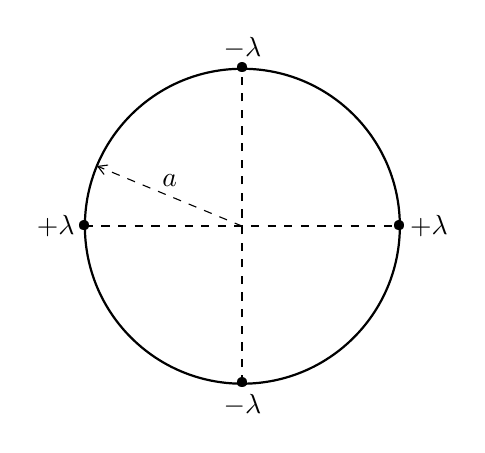
\begin{tikzpicture}[baseline, x=0.2cm, y=0.2cm]
            % axes
            \draw[dashed, thick] (0,-10) node[below] {$- \lambda$} -- (0,10) node[above] {$- \lambda$};
            \draw[dashed, thick] (-10, 0) node[left] {$+ \lambda$} -- (10,0) node[right] {$+ \lambda$};

            % points
            \foreach \Point in {(10,0), (0,10), (-10, 0), (0, -10)}{
                \node at \Point {\textbullet};
            }

            % circle
            \draw[thick] (0,0) circle (10);

            % radius
            \draw[dashed, arrows={-angle 60}] (0,0) -- (-9.239,3.827);
            \node[anchor=south] at (-4.619, 1.913) {$a$};
        \end{tikzpicture}
      \end{figure}
      \begin{figure}[H]
        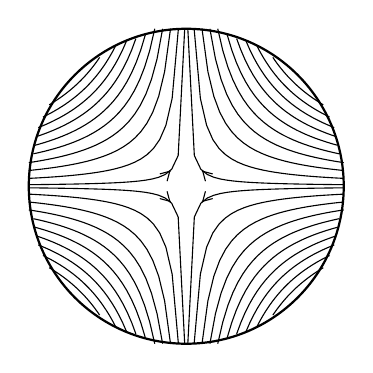
\begin{tikzpicture}[baseline, x=0.2cm, y=0.2cm]
            % circle
            \draw[thick] (0,0) circle (10);

            % Field lines
            % Bottom left
            \draw plot[domain=-10.0:-0.1]   ({\x},{ 1 / \x});
            \draw plot[domain=-10.0:-0.5]   ({\x},{ 5 / \x});
            \draw plot[domain=-10.0:-1.0]   ({\x},{10 / \x});
            \draw plot[domain=-10.0:-1.5]   ({\x},{15 / \x});
            \draw plot[domain=-9.7 :-2.0]   ({\x},{20 / \x});
            \draw plot[domain=-9.6 :-2.6]   ({\x},{25 / \x});
            \draw plot[domain=-9.5 :-3.2]   ({\x},{30 / \x});
            \draw plot[domain=-9.4 :-3.8]   ({\x},{35 / \x});
            \draw plot[domain=-9.1 :-4.5]   ({\x},{40 / \x});
            \draw plot[domain=-8.7 :-5.5]   ({\x},{45 / \x});

            % Top right
            \draw plot[domain=10.0:0.1]   ({\x},{ 1 / \x});
            \draw plot[domain=10.0:0.5]   ({\x},{ 5 / \x});
            \draw plot[domain=10.0:1.0]   ({\x},{10 / \x});
            \draw plot[domain=10.0:1.5]   ({\x},{15 / \x});
            \draw plot[domain=9.7 :2.0]   ({\x},{20 / \x});
            \draw plot[domain=9.6 :2.6]   ({\x},{25 / \x});
            \draw plot[domain=9.5 :3.2]   ({\x},{30 / \x});
            \draw plot[domain=9.4 :3.8]   ({\x},{35 / \x});
            \draw plot[domain=9.1 :4.5]   ({\x},{40 / \x});
            \draw plot[domain=8.7 :5.5]   ({\x},{45 / \x});

            % Top left
            \draw plot[domain=-10.0:-0.1]   ({\x},{- 1 / \x});
            \draw plot[domain=-10.0:-0.5]   ({\x},{- 5 / \x});
            \draw plot[domain=-10.0:-1.0]   ({\x},{-10 / \x});
            \draw plot[domain=-10.0:-1.5]   ({\x},{-15 / \x});
            \draw plot[domain=-9.7 :-2.0]   ({\x},{-20 / \x});
            \draw plot[domain=-9.6 :-2.6]   ({\x},{-25 / \x});
            \draw plot[domain=-9.5 :-3.2]   ({\x},{-30 / \x});
            \draw plot[domain=-9.4 :-3.8]   ({\x},{-35 / \x});
            \draw plot[domain=-9.1 :-4.5]   ({\x},{-40 / \x});
            \draw plot[domain=-8.7 :-5.5]   ({\x},{-45 / \x});

            % Top right
            \draw plot[domain=10.0:0.1]   ({\x},{- 1 / \x});
            \draw plot[domain=10.0:0.5]   ({\x},{- 5 / \x});
            \draw plot[domain=10.0:1.0]   ({\x},{-10 / \x});
            \draw plot[domain=10.0:1.5]   ({\x},{-15 / \x});
            \draw plot[domain=9.7 :2.0]   ({\x},{-20 / \x});
            \draw plot[domain=9.6 :2.6]   ({\x},{-25 / \x});
            \draw plot[domain=9.5 :3.2]   ({\x},{-30 / \x});
            \draw plot[domain=9.4 :3.8]   ({\x},{-35 / \x});
            \draw plot[domain=9.1 :4.5]   ({\x},{-40 / \x});
            \draw plot[domain=8.7 :5.5]   ({\x},{-45 / \x});

            \draw[arrows={angle 60-}] (.999, 1.001) -- (1.001, 0.999);
            \draw[arrows={angle 60-}] (.999, -1.001) -- (1.001, -0.999);
            \draw[arrows={angle 60-}] (-.999, 1.001) -- (-1.001, 0.999);
            \draw[arrows={angle 60-}] (-.999, -1.001) -- (-1.001, -0.999);
            \end{tikzpicture}
          \end{figure}
            The charge density in two dimensions can be expressed as
            \begin{align*}
                \sigma(\varrho, \phi) =
                \frac{\lambda}{a}
                \sum_{n=0}^3 {\left(-1\right)}^n \delta(\varrho - a) \delta\left(\phi - \frac{n \pi}{2}\right)
            \end{align*}
            \begin{enumerate}
                \item
                    Using the Green function expansion from Problem 2.17c, show that the electrostatic potential is
                    \begin{align*}
                        \Phi(\varrho, \phi) =
                        \frac{\lambda}{\pi \epsilon_0}
                        \sum_{k=0}^\infty \frac{1}{2 k + 1}
                        {\left(
                            \frac{\varrho_<}{\varrho_>}
                        \right)}^{4k + 2}
                        \cos\left[(4k + 2) \phi \right]
                    \end{align*}
                    \begin{sol}
                        \begin{align*}
                            \Phi(\varrho, \phi) &= \frac{1}{4 \pi \epsilon_0}\int_\Omega
                            \sigma(\varrho', \phi')G(\varrho, \phi; \varrho', \phi') \varrho d\varrho d\phi
                            \\
                            &= \frac{\lambda}{4 \pi \epsilon_0}
                            \sum_{n = 0}^{3}{(-1)}^n
                            \left\{
                                -\ln(\varrho_>^2) +
                                2 \sum_{m = 1}^{\infty}\frac{1}{m}
                                {\left(
                                    \frac{\varrho_<}{\varrho_>}
                                \right)}^m
                                \cos\left[m (\phi - \frac{n \pi}{2})\right]
                            \right\}
                            \\
                            &= \frac{\lambda}{2 \pi \epsilon_0}
                            \sum_{m = 1}^{\infty}\frac{1}{m}
                            {\left(
                                \frac{\varrho_<}{\varrho_>}
                            \right)}^m
                            \sum_{n = 0}^{3}{(-1)}^n
                            \cos\left[m (\phi - \frac{n \pi}{2})\right]
                        \end{align*}
                        Since the $\ln$ term cancels after summing over $n$
                        \\
                        Expanding the second sum yields:
                        \begin{align*}
                            \sum_{n = 0}^{3}{(-1)}^n
                            &\cos\left[m (\phi - \frac{n \pi}{2})\right]
                            \\
                            &=
                            \cos(m \phi) - \cos \left(m \phi - \frac{m \pi}{2}\right)
                            + \cos \left(m \phi - m \pi\right)
                            - \cos \left(m \phi - \frac{3 m \pi}{2}\right)
                            \\
                            &= \cos(m\phi) - \cos(m\phi)\cos\left(\frac{m\pi}{2}\right)
                            + \sin(m \phi)\sin\left(\frac{m \pi}{2}\right) + \cdots
                        \end{align*}
                        The first two terms show that $m$ must be a
                        multiple of 2, and the second two show that it
                        must be an odd multiple of 2 (otherwise the
                        sum is 0):
                        \begin{align*}
                            \sum_{n = 0}^{3}{(-1)}^n
                            \cos\left[m (\phi - \frac{n \pi}{2})\right]
                            = 2 \cos (m \phi)
                            \\
                            \text{for }
                            m = 2 (2k + 1) = 4k + 2
                        \end{align*}
                        \begin{align*}
                            \Phi(\varrho, \phi) &= \frac{\lambda}{\pi \epsilon_0}
                            \sum_{k = 0}^{\infty}\frac{1}{2k + 1}
                            {\left(
                                \frac{\varrho_<}{\varrho_>}
                            \right)}^{4k + 2}
                            \cos\left[ (4k + 2) \phi \right]
                        \end{align*}
                    \end{sol}
                \item
                    Relate the solution of part a to the real part of the complex function
                    \begin{align*}
                        w(z) = \frac{2 \lambda}{4 \pi \epsilon_0} \ln \left[ \frac{(z-ia)(z+ia)}{(z-a)(z+a)} \right]
                    \end{align*}
                    where $z = x + iy = \varrho e^{i \phi}$. Comment on
                    the connection to Problem 2.3
                    \begin{sol}
                        \begin{align*}
                            \Phi(\varrho, \phi) &=
                            \frac{\lambda}{\pi \epsilon_0}
                            \sum_{k = 0}^{\infty}\frac{1}{2k + 1}
                            {\left(
                                \frac{\varrho_<}{\varrho_>}
                            \right)}^{4k + 2}
                            \cos\left[ (4k + 2) \phi \right]
                            \\
                            &= \Re
                            \left\{
                                \frac{2\lambda}{ \pi \epsilon_0}
                                \sum_{k = 0}^{\infty}\frac{1}{4k + 2}
                                {\left(
                                    \frac{\varrho_<}{\varrho_>}
                                    e^{i\phi}
                                \right)}^{4k + 2}
                            \right\}
                        \end{align*}
                        Since
                        \begin{align*}
                            \sum_{n \text{ odd}} \frac{Z^n}{n} = \frac{1}{2}\ln\left(\frac{1 + Z}{1 - Z}\right)
                        \end{align*}
                        \begin{align*}
                            \Rightarrow
                            \Phi(\varrho, \phi)
                            &=
                            \frac{\lambda}{2 \pi \epsilon_0}
                            \Re
                            \left\{
                            \ln
                                \left[
                                    \frac
                                    {
                                    1 + {\left( \dfrac{\varrho_>}{\varrho_<}e^{i\phi} \right)}^2
                                    }{
                                    1 - {\left( \dfrac{\varrho_>}{\varrho_<}e^{i\phi} \right)}^2
                                    }
                                \right]
                            \right\}
                            \\
                            &=
                            \frac{\lambda}{2 \pi \epsilon_0}
                            \Re
                            \left\{
                            \ln
                                \left[
                                    \frac
                                    {
                                    \left(1 + i\dfrac{\varrho_>}{\varrho_<}e^{i\phi}\right)
                                    \left(1 - i\dfrac{\varrho_>}{\varrho_<}e^{i\phi}\right)
                                    }{
                                    \left(1 + \dfrac{\varrho_>}{\varrho_<}e^{i\phi}\right)
                                    \left(1 - \dfrac{\varrho_>}{\varrho_<}e^{i\phi}\right)
                                    }
                                \right]
                            \right\}
                        \end{align*}
                        The interior solution has $\varrho_< = \varrho$
                        and $\varrho_> = a$ so the solution becomes
                        \begin{align*}
                            \Phi(\varrho, \phi) &=
                            \frac{\lambda}{2 \pi \epsilon_0}
                            \Re
                            \left\{
                            \ln
                                \left[
                                    \frac
                                    {
                                    \left(\varrho + iae^{i\phi}\right)
                                    \left(\varrho - iae^{i\phi}\right)
                                    }{
                                    \left(\varrho + ae^{i\phi}\right)
                                    \left(\varrho - ae^{i\phi}\right)
                                    }
                                \right]
                            \right\}
                            \\
                            &= \Re \left[ w(\varrho) \right]
                        \end{align*}
                        The exterior solution has $\varrho_> = \varrho$
                        and $\varrho_< = a$ so the solution becomes
                        \begin{align*}
                            \Phi(\varrho, \phi) &=
                            \frac{\lambda}{2 \pi \epsilon_0}
                            \Re
                            \left\{
                            \ln
                                \left[
                                    \frac
                                    {
                                    \left(i\varrho + ae^{i\phi}\right)
                                    \left(i\varrho - ae^{i\phi}\right)
                                    }{
                                    \left(\varrho + ae^{i\phi}\right)
                                    \left(\varrho - ae^{i\phi}\right)
                                    }
                                \right]
                            \right\}
                        \end{align*}
                        Multiply the fraction by $i^2$ to obtain
                        $\Phi = \Re\left[w(\varrho)\right]$
                        \\
                        This is related to problem 2.3 since that
                        problem can be solved with the original line
                        charge and 3 image charges, corresponding to
                        the 4 line charges surrounding the
                        accelerator. Simply take one of the line
                        charges to be at $(x_0, y_0)$ where $x_0 =
                        y_0$
                    \end{sol}
                \item
                    Find expressions for the Cartesian components of
                    the electric field near the origin, expressed in
                    terms of x and y. Keep the $k = 0$ and $k = 1$
                    terms in the expansion. For $y = 0$ what is the
                    relative magnitude of the $k = 1$ ($2^6$-pole)
                    contribution to $E_x$ compared to the $k=0$
                    ($2^2$-pole or quadrupole) term?
                    \begin{sol}
                        The Cartesian components of the electric field are given by
                        \begin{align*}
                            E_x = -\cos{\theta} \frac{\partial \Phi}{\partial \varrho}
                            + \frac{\sin{\theta}}{\varrho}\frac{\partial \Phi}{\partial \phi}
                            \\
                            E_y = -\sin{\theta} \frac{\partial \Phi}{\partial \varrho}
                            - \frac{\cos{\theta}}{\varrho}\frac{\partial \Phi}{\partial \phi}
                        \end{align*}
                        For $\varrho < a$ we have
                        \begin{align*}
                            \frac{\partial \Phi}{\partial \varrho}
                            &=
                            \frac{2 \lambda}{a \pi \epsilon_0}
                            \sum_{k=0}^{\infty}{\left(\frac{\varrho}{a}\right)}^{4k+1}\cos\left[\phi(4k + 2)\right]
                            \\
                            \frac{1}{\varrho}\frac{\partial \Phi}{\partial \phi}
                            &=
                            -\frac{2 \lambda}{a \pi \epsilon_0}
                            \sum_{k=0}^{\infty}{\left(\frac{\varrho}{a}\right)}^{4k+1}\sin\left[\phi(4k + 2)\right]
                        \end{align*}
                        Substituting into the original expressions for the components of $E$:
                        \begin{align*}
                            E_x &=
                            -\frac{2 \lambda}{a \pi \epsilon_0}
                            \sum_{k=0}^{\infty}
                            {\left(
                                \frac{\varrho}{a}
                            \right)}^{4k + 1}
                            \left\{
                                \cos\left[\phi \left(4k+2\right)\right]\cos\phi
                                +
                                \sin\left[\phi \left(4k+2\right)\right]\sin\phi
                            \right\}
                            \\
                            &=
                            \frac{2 \lambda}{a \pi \epsilon_0}
                            \sum_{k=0}^{\infty}
                            {\left(
                                \frac{\varrho}{a}
                            \right)}^{4k + 1}
                            \cos\left[\phi \left(4k+1\right)\right]
                            \\
                            E_y &=
                            -\frac{2 \lambda}{a \pi \epsilon_0}
                            \sum_{k=0}^{\infty}
                            {\left(
                                \frac{\varrho}{a}
                            \right)}^{4k + 1}
                            \left\{
                                -\sin\phi \cos\left[\phi \left(4k+2\right)\right]
                                -
                                \cos\phi \sin\left[\phi \left(4k+2\right)\right]
                            \right\}
                            \\
                            &=
                            \frac{2 \lambda}{a \pi \epsilon_0}
                            \sum_{k=0}^{\infty}
                            {\left(
                                \frac{\varrho}{a}
                            \right)}^{4k + 1}
                            \sin\left[\phi \left(4k+3\right)\right]
                        \end{align*}
                        Up to k = 1, this yields:
                        \begin{align*}
                            E_x &= \frac{2 \lambda}{a \pi \epsilon_0}
                            \left[
                                \frac{\varrho}{a}\cos\phi + {\left(\frac{\varrho}{a}\right)}^5\cos 5\phi
                            \right]
                            \\
                            E_y &= \frac{2 \lambda}{a \pi \epsilon_0}
                            \left[
                                \frac{\varrho}{a}\sin 3\phi + {\left(\frac{\varrho}{a}\right)}^5\sin 7\phi
                            \right]
                        \end{align*}
                        For $y = 0$, $\phi = 0, \pi$:
                        \begin{align*}
                            E_x &= \pm \frac{2 \lambda}{a \pi \epsilon_0}
                            \left[
                                \frac{\varrho}{a} \pm {\left(\frac{\varrho}{a}\right)}^5
                            \right]
                        \end{align*}
                        The relative strength of the $k=0$ and $k=1$ terms
                        is $\varrho^4$
                    \end{sol}
            \end{enumerate}
\end{enumerate}
\end{document}
